\documentclass[11pt]{article}
\usepackage[margin=1in]{geometry}
\usepackage[expansion=false]{microtype}
\usepackage{amsmath,amssymb}
\usepackage{graphicx}
\usepackage{booktabs}
\usepackage{tabularx}
\usepackage{enumitem}
\usepackage{xcolor}
\usepackage[colorlinks=true,linkcolor=blue,urlcolor=blue]{hyperref}
\graphicspath{{figures/}}
% \code: typewriter text that may line-break after an underscore
\newcommand{\code}[1]{\texttt{\begingroup\def\_{\textunderscore\allowbreak}#1\endgroup}}
\pdfstringdefDisableCommands{\def\code#1{#1}}
\newcommand{\btn}[1]{\textsf{\textbf{#1}}}   % a GUI button or control
\usepackage{tikz}
% \mk{n}: the red numbered marker drawn on the screenshots
\DeclareRobustCommand{\mk}[1]{\tikz[baseline=(m.base)]\node[circle,fill=red!80!black,text=white,inner sep=1.2pt,
  minimum size=1.15em,font=\sffamily\bfseries\footnotesize](m){#1};}
\setlength{\emergencystretch}{3em}
\setlist{itemsep=2pt,topsep=3pt}

\title{\textbf{NMR Tuning and Operation}\\[4pt]
\large Quadrature Phase Tunes, Auto Tune and the New Run Controls in PyNMR (UNH fork)}
\author{UNH Polarized Target Group}
\date{\today}

\begin{document}
\maketitle

\begin{center}
\fbox{\parbox{0.85\textwidth}{\centering
\textbf{Note on provenance.} This document was drafted with AI assistance (Claude),
under the direction of and with technical input from E. Long. It has not undergone
the review process required for publication and may contain errors, gaps, or
outdated statements. It is included here because it is useful for understanding and
running the accompanying code, not as a citable or publication-ready reference.}}
\end{center}
\bigskip

\begin{abstract}
This note is the operator's guide to the tuning and quadrature features added to PyNMR in the UNH fork
(\code{unhpoltarg/jlab\_pynmr}) during October--November 2026. PyNMR can now record both quadratures of the
deuteron NMR signal, absorption (Real, $0^\circ$) and dispersion (Imag, $90^\circ$), by stepping the phase
detector's reference between events, optionally with the opposite-sign settings $180^\circ$ and $270^\circ$
that cancel detector offsets. The operator sets each phase tune roughly by eye; \btn{Auto Tune} then moves
them to the true angles using only the background Q-curve, in about 50~s for a Real/Imag pair. The note
covers starting PyNMR safely, tuning, taking quadrature data, what lands in which file, and what to do when
something goes wrong. An appendix explains why the Q-curve alone fixes the absorptive phase: at every
frequency the NMR absorption points along the normal to the Q-curve's trace in the complex plane, which is
the origin of the empirical form $\theta(f)=\theta_0+2\arctan\!\big((f-f_0)/\gamma\big)$. Everything here has been
checked against the built-in simulator. \textbf{Auto Tune, the split plots, the per-angle baselines, the
dispersive background and the $64\times N$ sweep controls have not yet been run on the Hall~B box.}
\end{abstract}


%=====================================================================================================
\section*{Quick Start Guide}
\addcontentsline{toc}{section}{Quick Start Guide}
\label{sec:quick}
For operators who have done this before. Each red number \mk{n} on the screenshots (Figs.~\ref{fig:qs-tune}--\ref{fig:qs-base})
is the step with that number. Everything after this guide is background and detail.

\begin{enumerate}[leftmargin=2.2em,itemsep=3pt]
\item \textbf{Start PyNMR} on the DAQ computer, then start the online fitter if you use it:
\begin{verbatim}
conda deactivate          # repeat until no environment is active
conda activate pynmr312
python pynmr_main.py -p Deuteron
\end{verbatim}
\item \mk{2} \textbf{Run tab:} set \btn{Center Freq} (the Larmor frequency) and \btn{Half-width}, then \btn{Apply Window}.
  (In the \code{TestSimQuad} simulator the \btn{Event Label} also drives the target: None/Baseline, TE, Polarize, Junk.)
\item \mk{3} \textbf{Sweeps per Event} $=64\times N$: \btn{Unlock}, set $N$ (default 1), \btn{Set}.
\item \mk{4} \textbf{Tune tab:} \btn{Run} the tune loop and tune the tank with \btn{Diode Tune Control}.
\item \mk{5} \textbf{Rough phase tunes} (optional): Auto Tune maps the whole phase-DAC range first, so it needs no
  hand tunes. The Real tune is its phase reference, and the very first time the Imag tune tells it which
  dispersive side to call $90^\circ$; after that the side is kept. Last cooldown's tunes are loaded as defaults.
\item \mk{6} \textbf{Auto Tune} (about 70~s for Real/Imag, 2~min for cycle4; the tune loop pauses and restarts by itself). While it scans,
  \btn{Phase Tune Control} shows the setting being measured and the tune controls are locked; at the end
  it shows the new tune.
\item \mk{7} \textbf{Check} the result line (how far each tune was off, $\pm$ error) and the trace plot. Wrong?
  \btn{Undo Auto Tune}.
\item \mk{8} \textbf{Auto Calibrate Phase} (about 90~s), only at the start of a cooldown, after an RF hardware change,
  or after the centre frequency moved by more than 0.05~MHz.
\item[] \textbf{Sign:} at the true $0^\circ$ (diode smile, phase frown) positive P is a downward line. Take a TE there
  before trusting P: a CC from the old $180^\circ$ setting has the wrong sign (\S\ref{sec:concepts}).
\item \mk{9} \textbf{Stop the tune loop.} On the Run tab choose the sequence (pair, abba or cycle4) and tick
  \btn{Quadrature}. If it won't tick, the reason is shown in red under it.
\item \mk{10} \textbf{Baseline run:} move the field so the line is out of the window, set Event Label to Baseline,
  \btn{Run} a few complete cycles, \btn{Stop}.
\item \mk{11} \textbf{Baseline tab:} \btn{Select Current Eventfile}; select the whole baseline run (click its first row,
  shift-click its last); read the summary line; \btn{Set Baseline}.
\item \mk{12} \textbf{Run tab:} the \btn{Baselines} line must say ok for every angle.
\item \textbf{Take data:} field back on the line, Event Label as needed, \btn{Run}.
\item \mk{14} \textbf{Wing bins} (on Baseline Subtracted Real): adjust until the dashed red part of the yellow fit stays
  clear of the line.
\item \textbf{Stop} with \btn{Stop}. If the exit dialog appears, choose \btn{Abort! I didn't mean to make this appear!}
\end{enumerate}
Also: a TE (\S\ref{sec:te}); the Analysis tab (\S\ref{sec:analysis}); anything in red (\S\ref{sec:trouble}).

\begin{figure}[p]
\centering
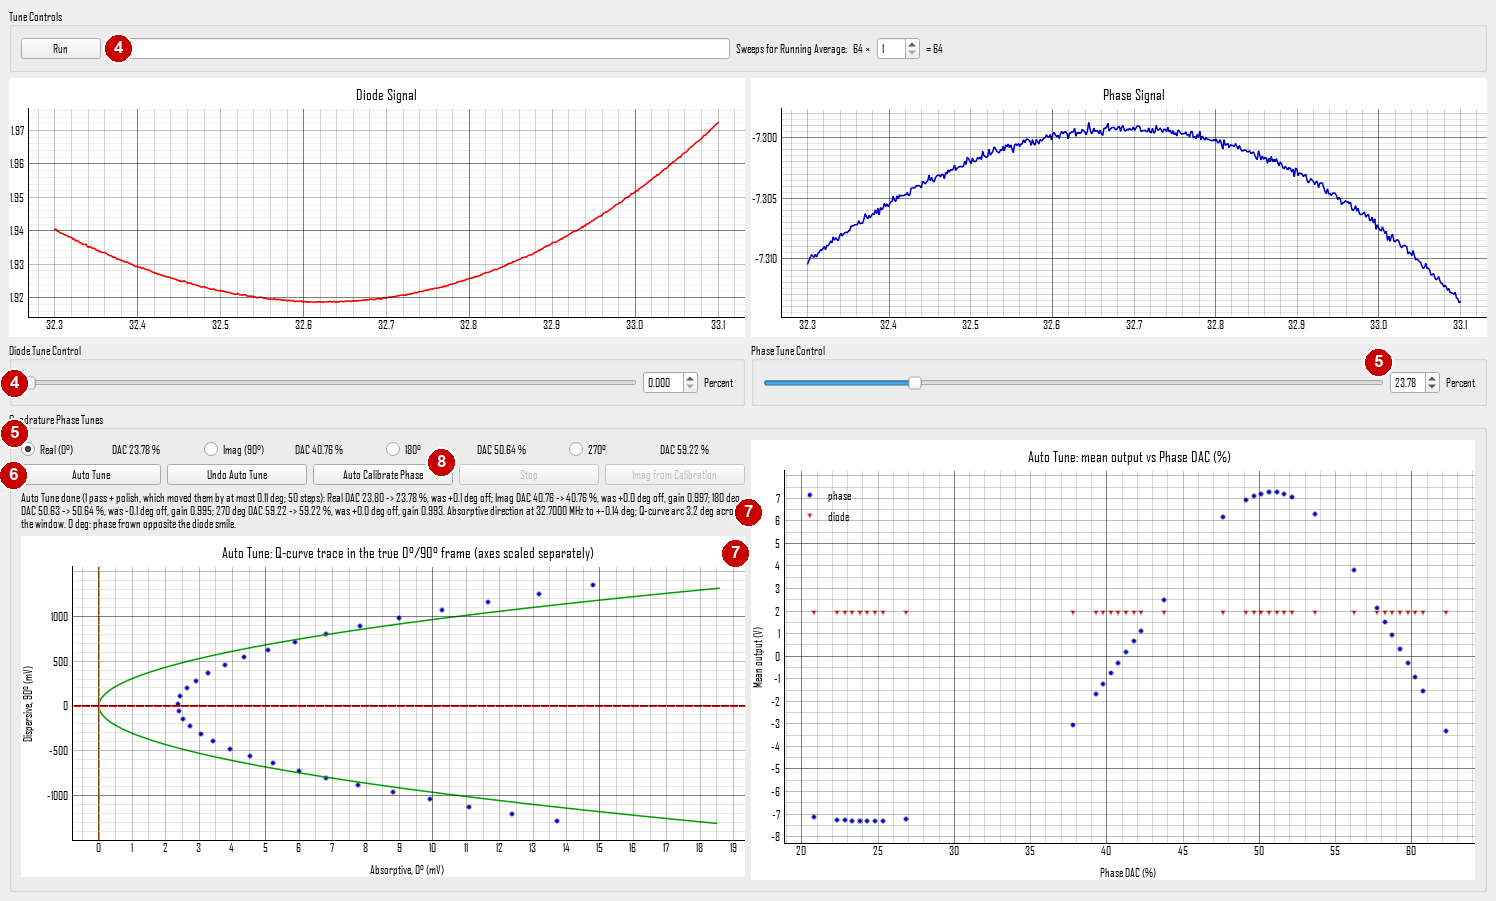
\includegraphics[width=\textwidth]{qs_tune_marked.png}
\caption{Quick Start, Tune tab. \mk{4} \btn{Run} the tune loop; \btn{Diode Tune Control}. \mk{5} the tune selector
(\btn{Real (0°)}, \btn{Imag (90°)}, $180^\circ$, $270^\circ$, each with its phase DAC setting) and the \btn{Phase Tune} box.
\mk{6} \btn{Auto Tune} (\btn{Undo Auto Tune} beside it). \mk{7} the result line and, under it, the trace plot (red
dashes: the $0^\circ$ direction; orange: $90^\circ$). \mk{8} \btn{Auto Calibrate Phase}. Right: mean output against
phase DAC for the scan.}
\label{fig:qs-tune}
\vspace{1em}
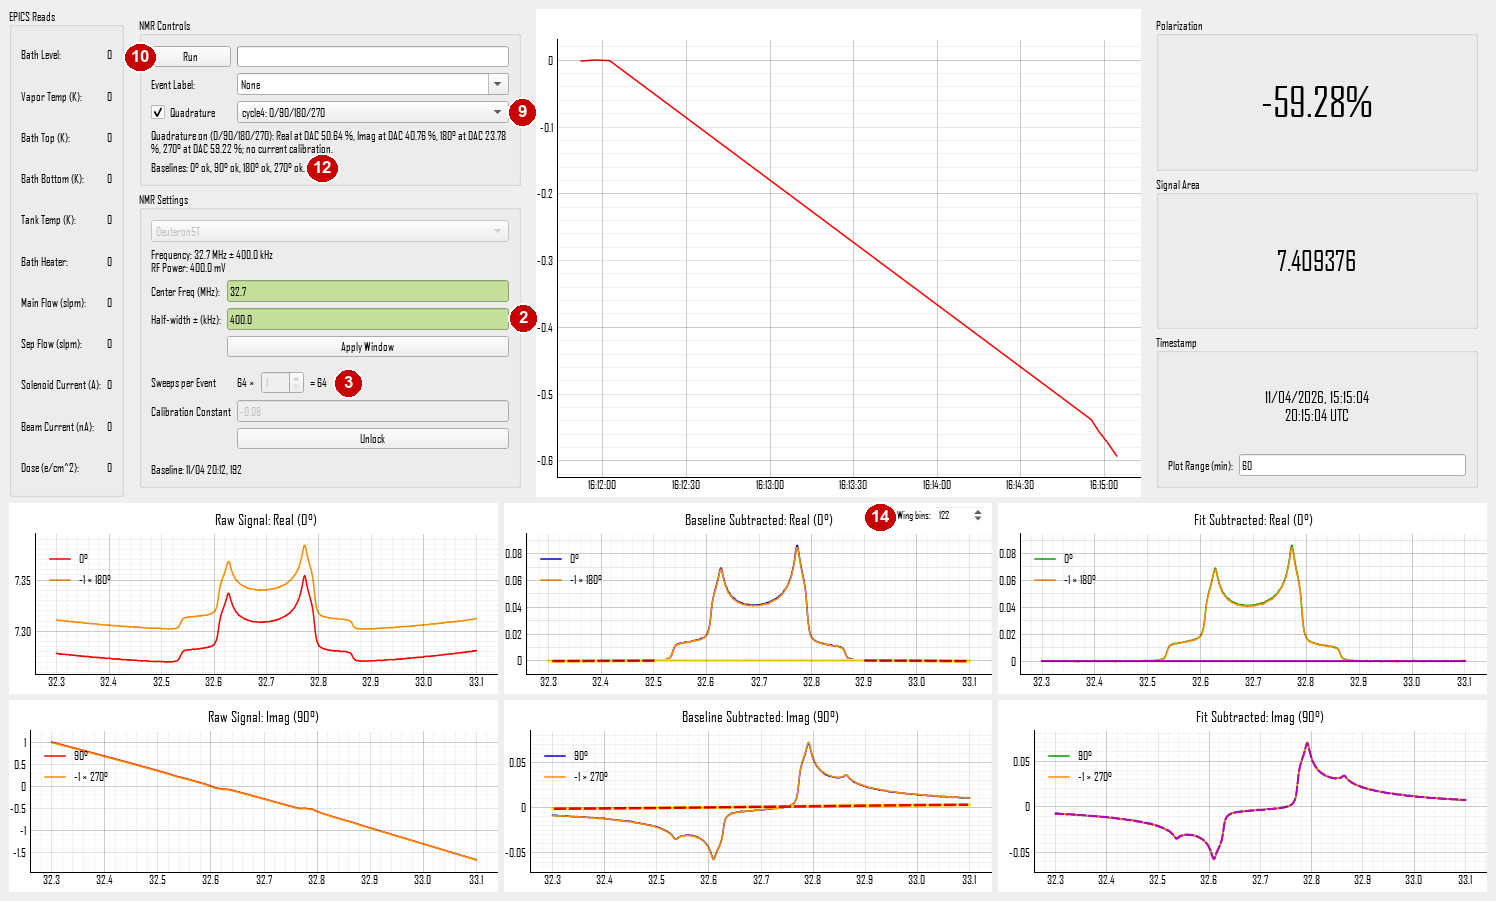
\includegraphics[width=\textwidth]{qs_run_marked.png}
\caption{Quick Start, Run tab (cycle4 run, simulator). \mk{2} window: \btn{Center Freq}, \btn{Half-width},
\btn{Apply Window}. \mk{3} Sweeps per Event $64\times N$. \mk{9} \btn{Quadrature} and the sequence. \mk{10} \btn{Run}.
\mk{12} the \btn{Baselines} line. \mk{14} \btn{Wing bins}, with the fitted points dashed red on the yellow fit.}
\label{fig:qs-run}
\end{figure}

\begin{figure}[ht]
\centering
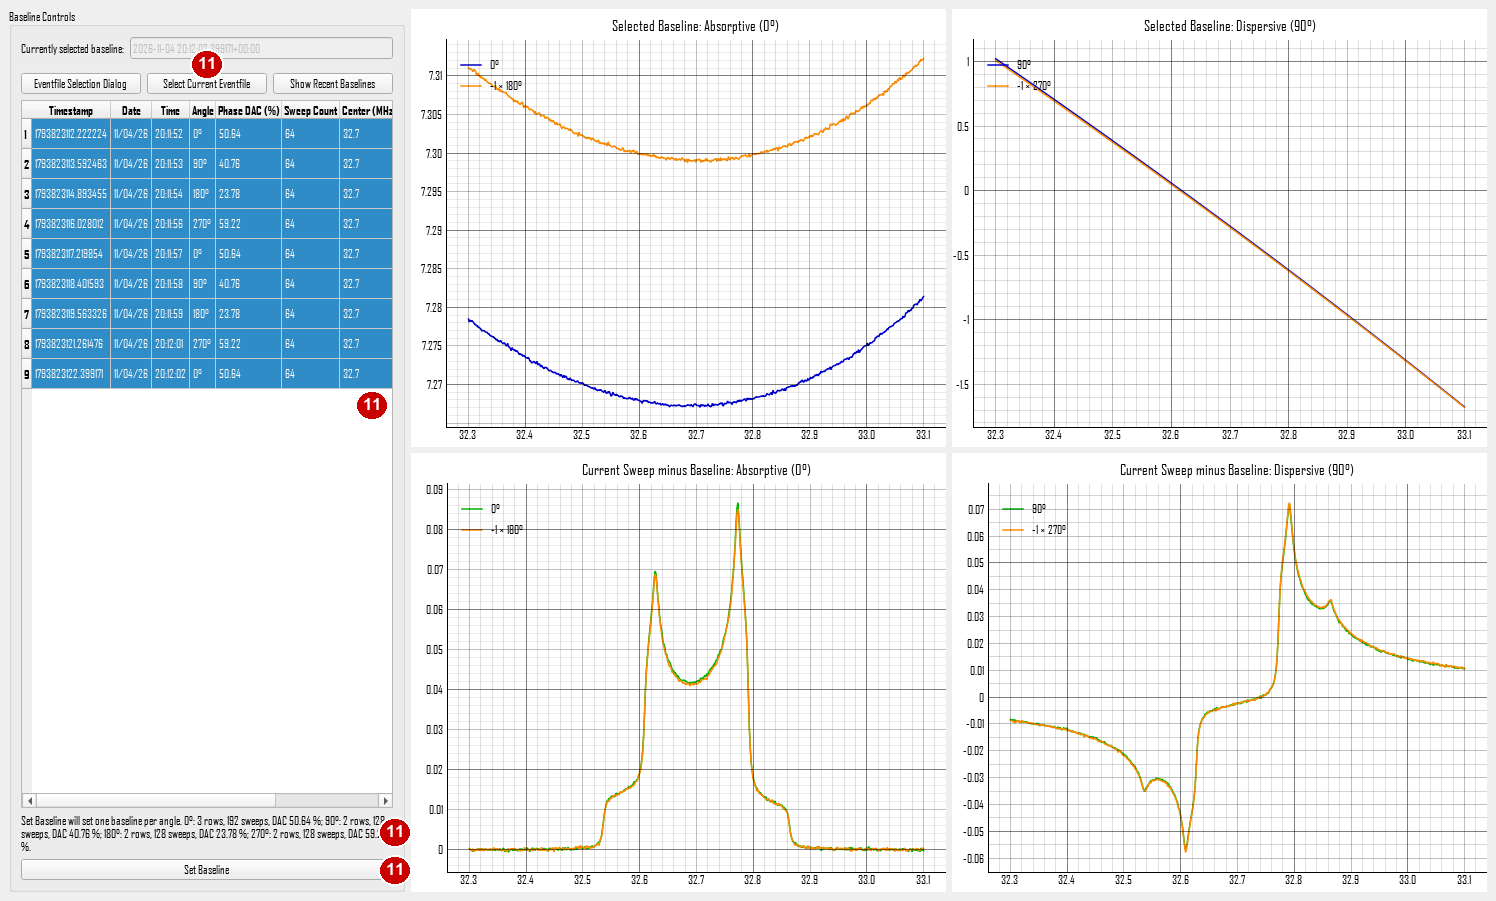
\includegraphics[width=\textwidth]{qs_base_marked.png}
\caption{Quick Start, Baseline tab. \mk{11} \btn{Select Current Eventfile}; select all rows of the baseline run (the
Angle and Phase DAC columns show each row's setting); check the summary line above \btn{Set Baseline}; click it.
Right: each angle's baseline (top) and the current sweep minus it (bottom), absorptive left, dispersive right.}
\label{fig:qs-base}
\end{figure}
\clearpage
\tableofcontents
\bigskip

%=====================================================================================================
\section{What is new}
\label{sec:new}

\begin{table}[ht]
\centering\small
\begin{tabularx}{\textwidth}{@{}lXl@{}}
\toprule
Feature & What it does for the operator & Where \\
\midrule
Python 3.12 env & PyNMR on the DAQ computer runs in \code{pynmr312}; the old 3.11 env crashed mid-run & \S\ref{sec:start} \\
Box connections & Each event closes its connection to the FPGA box cleanly; the box is told to stop after errors & \S\ref{sec:start} \\
Data streamer & Each finished $0^\circ$ event goes to the online fitter; on by default & \S\ref{sec:start} \\
NMR window & Centre frequency and half-width set from the Run tab, between events & \S\ref{sec:window} \\
$64\times N$ sweeps & Sweeps per event and the Tune running average are whole 64-sweep chunks & \S\ref{sec:sweeps} \\
Wing points & The wing fit's size as points per side, with the fitted points marked & \S\ref{sec:wings} \\
Phase tunes & Separate Real, Imag, $180^\circ$ and $270^\circ$ tunes on the Tune tab & \S\ref{sec:tuning} \\
\btn{Auto Tune} & Refines the hand tunes to the true angles from the Q-curve & \S\ref{sec:autotune} \\
\btn{Auto Calibrate Phase} & Measures the phase shifter over its whole range & \S\ref{sec:cal} \\
Quadrature runs & Events alternate between tunes: pair, abba or cycle4 & \S\ref{sec:run} \\
Quadrature baselines & One selection of a baseline run gives each angle its own baseline & \S\ref{sec:baselines} \\
Dispersive background & $90^\circ$/$270^\circ$ records: background fitted jointly with KK of the absorption & \S\ref{sec:disp} \\
Quadrature plots & A $2\times3$ grid: each processing stage split into $0^\circ$ and $90^\circ$ & \S\ref{sec:plots} \\
\bottomrule
\end{tabularx}
\caption{The new features and where they are described.}
\label{tab:new}
\end{table}

All UNH code lives in \code{unh/}; every change to a JLab file is marked with a \code{UNH-HOOK} label and
can be removed with \code{python -m unh.strip\_unh}. The quadrature code is in \code{unh/quadrature/},
its settings in \code{unh/quadrature/quadrature.yaml}, and its design notes in
\code{notes/quadrature\_phase\_design.md}.

%=====================================================================================================
\section{Before you start}
\label{sec:start}

\paragraph{Use the Python 3.12 environment.} On the DAQ computer (Linux/WSL):
\begin{verbatim}
conda deactivate          # repeat until no environment is active
conda activate pynmr312
python --version          # must say 3.12 or newer
python pynmr_main.py -p Deuteron
\end{verbatim}
On the old Python~3.11 environment PyNMR died silently in the middle of runs, most often with the
streamer on. The cause was \code{Fatal Python error: none\_dealloc}, raised while pyqtgraph redrew the plots;
Python~3.12 cannot raise it. Stacked conda environments can leave the old Python first on the path, hence
the \code{conda deactivate}. The fitter should also run on Python~3.12.

\paragraph{Never kill PyNMR in the middle of a sweep.} The deuteron box (192.168.0.72) stops answering, even
on UDP, if PyNMR dies while the box is sweeping, and only a power cycle brings it back. Stop runs with the
\btn{Run}/\btn{Stop} button and close PyNMR normally. If you close PyNMR while the Run loop is on, it asks first: choose
\btn{Abort! I didn't mean to make this appear!} to keep running; \btn{Ignore. I am an expert and I understand the
consequences.} closes it mid-sweep. There is no such warning for the Tune loop, \btn{Auto Tune} or
\btn{Auto Calibrate Phase}: stop those before closing. PyNMR now closes every connection cleanly and sends the
stop-sweep command after errors and at the end of tuning; on the DAQ computer this cut the connection time
from 2.0~s to under 0.2~s per event.

\paragraph{The online fitter.} The data streamer is on by default (\code{unh/data\_streamer.yaml},
\code{enable: True}). It sends each finished deuteron event's fit-subtracted line to LabView-NMR-Fitter on
\code{127.0.0.1:8777}. If the fitter isn't running, PyNMR logs one warning per outage and carries on; it
never waits for the fitter. In quadrature runs only the $0^\circ$ records are sent.

\paragraph{Turning quadrature on for a profile.} The quadrature controls appear only for profiles enabled in
\code{unh/quadrature/quadrature.yaml}. \code{Deuteron} and the simulator profile \code{TestSimQuad} have them on
(another profile is added the same way):
\begin{verbatim}
profiles:
    Deuteron:
        enable: True
\end{verbatim}
TestSimQuad and runs with no hardware:
\code{python pynmr\_main.py -p TestSimQuad}. In it the Run tab's \btn{Event Label} decides what the simulated target
does: \emph{None} or \emph{Baseline}, the line moved out of the window (P relaxes towards TE); \emph{TE}, thermal
equilibrium at 5~T and 1~K (about 0.1\,\%); \emph{Polarize}, a spin-up from wherever P is; \emph{Junk}, a very noisy,
bouncing line that is useless for anything. The simulator has no temperature reading, so a TE can't be completed
on the TE tab there.

%=====================================================================================================
\section{Concepts}
\label{sec:concepts}

\paragraph{Phase-sensitive detection.} The Q-meter's phase channel multiplies the tank voltage $V$ by a
reference of phase $\phi$ and keeps $P_\phi=g\,\mathrm{Re}\!\big(V e^{-i\phi}\big)+o$, where $g$ is the
detector gain and $o$ a DC offset. With the reference on the absorptive direction the output is the
absorption $\chi''$ (\textbf{Real, $0^\circ$}); a quarter turn later it is the dispersion $\chi'$
(\textbf{Imag, $90^\circ$}). At $180^\circ$ and $270^\circ$ the signal flips sign but the offset $o$ does
not, so the pair differences
\begin{equation}
  I=\tfrac12\big(P_{0}-P_{180}\big),\qquad Q=\tfrac12\big(P_{90}-P_{270}\big)
  \label{eq:pairs}
\end{equation}
are free of detector offsets.

\paragraph{Which way is $0^\circ$: the UNH sign convention (E.~Long, 2026-11-04).} For the deuteron the $m=+1$ level
is lowest, $0$ in the middle and $-1$ highest. With positive P the spin system takes energy from the RF, so at the
true $0^\circ$ setting a positive polarization gives a \emph{dip}, a downward-pointing line, and a negative
polarization an upward one. On this Q-meter that $0^\circ$ setting is the one where the phase Q-curve is a
\textbf{frown} while the diode is a \textbf{smile}. The 2026-10-27 data agree: at phase DAC 0.535--0.547 (frown) the
line pointed down, at 0.389--0.40 (smile) up. \textbf{Past UNH cooldowns ran at the $180^\circ$ setting} (smile),
with upward lines for positive P; their P values are still right wherever the CC came from a TE taken at the same
setting, because the CC carries the sign. Auto Tune now enforces the frown (\S\ref{sec:autotune}).
\begin{itemize}
\item \textbf{Take a new TE after moving to the true $0^\circ$.} A CC from a TE at the old $180^\circ$ setting has the
  wrong sign there, so P reads with the wrong sign until a TE is taken at the new setting.
\item The online fitter's McClellan model (and PyNMR's Optimized McClellan Fits) wants positive P as an \emph{upward}
  line, so the streamer flips the line before sending (\code{line\_sign: -1} in \code{unh/data\_streamer.yaml}).
  Set it to $+1$ only for data taken at the old setting. The TestSim profile keeps $+1$.
\item The TestSimQuad simulator has the UNH box's diode polarity (a smile) and starts on its frown side, so it
  behaves like the hardware.
\end{itemize}

\paragraph{The phase DAC.} The reference phase is set by a Mini-Circuits voltage-controlled phase shifter
(SCPHS-51+ on the deuteron box) driven by the box's phase DAC. The Tune tab shows the DAC setting as a
percentage of full scale, for example ``DAC 51.40\,\%''. \textbf{This is a control setting, not a fraction of
the signal.} The shifter covers about $456^\circ$ at 32.7~MHz, but its curve is S-shaped (a few degrees per
\% near 0, about $10^\circ$ per \% in the middle) and it stops responding above about 80\,\% DAC. The curve
also depends strongly on frequency: a calibration at 32.7~MHz is wrong at 22~MHz.

\paragraph{What the Q-curve can and can't tell.} As the frequency is swept, the Q-curve traces a curve in
the complex plane (a circle, or nearly a straight line for a heavily damped circuit). Appendix~\ref{app:normal}
shows that the NMR absorption at each frequency points along the normal to that trace. So the Q-curve alone
fixes the absorptive direction, and \btn{Auto Tune} uses that. Two things it can't fix are left to the hand
tunes: whether ``0'' is $\theta$ or $\theta+180^\circ$ (both are absorptive), and whether ``90'' is $+90^\circ$ or
$-90^\circ$ (the sign of the rotation isn't observable from projections). Auto Tune keeps whichever is nearer
the operator's hand setting.

\paragraph{The limit on $90^\circ$.} Projections determine the reference direction only up to a $2\times2$
linear map, so a $90^\circ$ angle needs one assumption: that the detector gain changes smoothly with the DAC
setting. $0^\circ$ and $180^\circ$ (antiparallel) don't need it. PyNMR's numbers are good for choosing and
monitoring the tunes; a $0.1^\circ$ phase should come from the offline complex lineshape fit, which uses the
Kramers--Kronig relation between $\chi'$ and $\chi''$.

%=====================================================================================================
\section{Setting up the NMR window and sweep counts}

\subsection{The NMR window}
\label{sec:window}
In NMR Settings on the Run tab, \btn{Center Freq (MHz)} and \btn{Half-width $\pm$ (kHz)} set the sweep window;
\btn{Apply Window} applies them. When PyNMR is idle the change is immediate; during a run it waits for the
next event. The half-width can go up to 5000~kHz in the deuteron profiles: the R\&S SMA100A's full FM deviation,
$r_m\times10$~MHz with $r_m=1/2$ for carriers up to 46.875~MHz (datasheet v06.01, p.~14). Its deviation accuracy is
specified up to half that, 2500~kHz. Other profiles keep 2000~kHz (\code{window\_limits: hw\_max\_khz} in
\code{pynmr\_config.yaml}). The window is saved in the session and restored at the next start. Keep the centre on the
deuteron Larmor frequency: \btn{Auto Tune} finds the absorptive phase at the centre frequency.

\subsection{Sweeps as $64\times N$}
\label{sec:sweeps}
The box delivers sweeps in chunks of 64, and when asked for 32 it returned 64. Sweep counts are therefore whole
chunks:
\begin{itemize}
\item \textbf{Run tab, Sweeps per Event:} $64\times N$, with $N$ set by the operator (default 1, i.e.\ 64
  sweeps). Press \btn{Unlock}, change $N$, press \btn{Set}, as before.
\item \textbf{Tune tab, Sweeps for Running Average:} $64\times N$, default $N=1$. Larger $N$ gives a smoother
  plot but makes it lag the knobs by about 1.8~s per chunk.
\item The tune chunk itself (\code{tune\_per\_chunk} in \code{pynmr\_config.yaml}) is 64 sweeps, so the Tune loop,
  \btn{Auto Tune} and \btn{Auto Calibrate Phase} all use 64-sweep chunks. A chunk takes about 1.8~s, so the
  tune connection waits up to 5~s for it (\code{timeout\_tune}; JLab's 1~s made the Tune loop stop after one try).
\end{itemize}

\subsection{The wing fit: points per side}
\label{sec:wings}
The yellow curve on Baseline Subtracted is JLab's \emph{Polynomial Fit to Wings} (3rd order by default),
which is subtracted to give Fit Subtracted. It is fitted to the outer parts of the sweep only. A box in the
title row of the Baseline Subtracted plot, \btn{Wing bins}, sets how many points (bins) it uses on \emph{each} side;
a dashed red curve on top of the yellow one marks exactly those points.
\begin{itemize}
\item The default is what the Analysis tab's fit bounds give (\code{analysis: wings} in \code{pynmr\_config.yaml}):
  148 points per side of 512 for the shared default 0.01/0.30/0.70/0.99, and 122 for the TestSim profiles.
  JLab's skip of the outermost 1\,\% on each side is kept.
\item Changing $N$ writes the Analysis tab's four bounds (they stay the one setting), redraws the last event's fit
  at once so the effect can be judged by eye, and applies to every event after it. Records already taken keep the
  fit they were analysed with.
\item Choose $N$ so the dashed red part stays clear of the line: too many points and the fit takes signal for
  background; too few and the polynomial is poorly pinned down.
\item In quadrature the box sits on the Baseline Subtracted Real plot. The $90^\circ$ plot is dashed over the whole
  sweep, because dispersive records use the joint KK fit (\S\ref{sec:disp}), not the wings.
\item $N$ goes back to the default when PyNMR restarts.
\end{itemize}

%=====================================================================================================
\section{Tuning}
\label{sec:tuning}

Figure~\ref{fig:tune} shows the Tune tab. Below the diode and phase plots, the \textbf{Quadrature Phase Tunes}
strip holds a selector for the tune being edited (Real, Imag, and $180^\circ$/$270^\circ$ when the sequence uses
them) with each tune's DAC setting, the buttons, a result line, and a small plot.

\begin{figure}[ht]
\centering
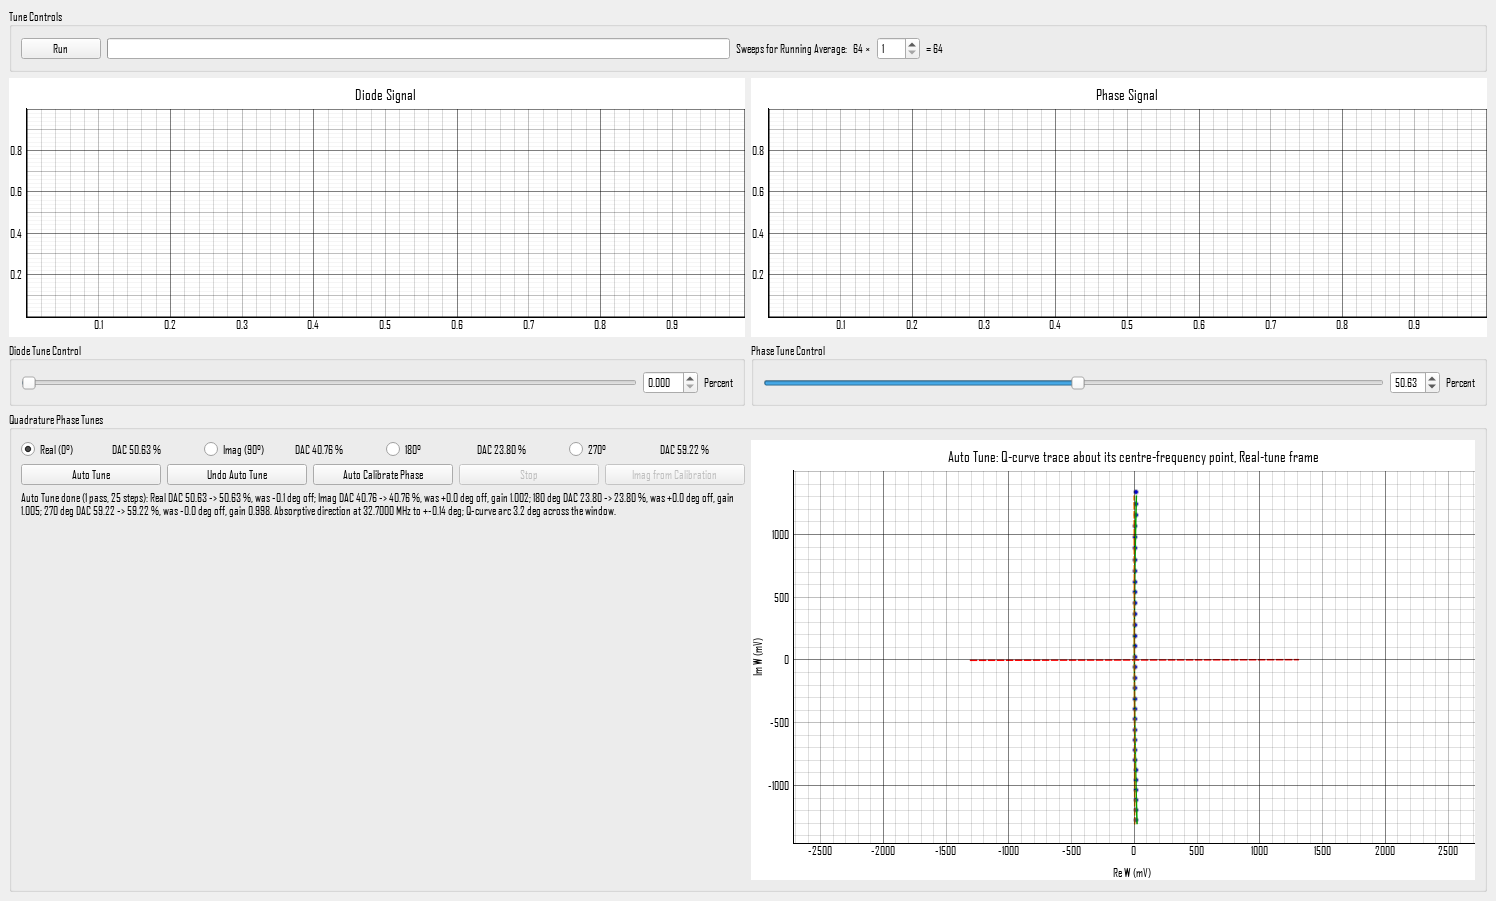
\includegraphics[width=\textwidth]{fig_tune_tab_autotune.png}
\caption{The Tune tab after a cycle4 \btn{Auto Tune} in the simulator. Bottom left: the tune selector with
each tune's DAC setting, the \btn{Auto Tune}, \btn{Undo Auto Tune}, \btn{Auto Calibrate Phase}, \btn{Stop} and
\btn{Imag from Calibration} buttons, and the result line; under it, once Auto Tune has a result, the Q-curve trace about its point
at the centre frequency, in the true $0^\circ$/$90^\circ$ frame Auto Tune found (absorptive across, dispersive up, each
axis scaled to its data so the bow shows), with the fit (green) and the $0^\circ$ (red) and $90^\circ$ (orange) axes
dashed. Bottom right: the mean output against the phase DAC for each step of the scan. The simulator's Q-meter is heavily damped, so its trace is nearly a straight line; the Hall~B tank
traces a visible circle (about $39^\circ$ of arc in the 2026-10-27 data).}
\label{fig:tune}
\end{figure}

\subsection{Tuning procedure}
\begin{enumerate}
\item Tune the tank (diode) as usual, with the Tune loop running (\btn{Run}).
\item Select \btn{Real (0°)} and set the Phase Tune by eye so the Q-curve looks absorptive. Roughly is
  enough: within about $30^\circ$.
\item Select \btn{Imag (90°)} and set its tune by eye, roughly a quarter turn away. For cycle4, also set
  $180^\circ$ and $270^\circ$, or leave them empty: with a current calibration (\S\ref{sec:cal}) PyNMR fills them
  opposite Real and Imag when cycle4 is turned on.
\item Click \btn{Auto Tune} (\S\ref{sec:autotune}). Check the result line and the plot.
\item Leave the selector on \btn{Real (0°)} when done; runs always restore the Real tune at the end.
\end{enumerate}

\paragraph{Starting values.} If the saved session has no usable set of tunes (one is missing, at DAC 0\,\%, or
on the Real tune), PyNMR starts from \code{default\_tunes} in \code{quadrature.yaml}. These are the settings of
the 2026-10-27 Hall~B cycle4 run at 32.511~MHz: Real 51.40\,\%, Imag 44.40\,\%, $180^\circ$ 30.39\,\%, $270^\circ$
60.31\,\%. That run's calibration put them at $0^\circ$, $-79.9^\circ$, $-180.0^\circ$ and $+100.0^\circ$, so Imag
and $270^\circ$ were about $10^\circ$ short of quadrature; \btn{Auto Tune} corrects that. A usable saved set (the
operator's latest) always wins.

\subsection{Auto Tune}
\label{sec:autotune}
\btn{Auto Tune} finds every tune the current sequence uses (Real and Imag, plus $180^\circ$ and $270^\circ$ for
cycle4) in one click. Since 2026-11-10 it starts with a coarse map (\code{autotune: map: True}):
\begin{enumerate}
\item It steps the phase DAC over its whole range (16 settings, with returns to the Real tune) and fits the result
  as a calibration: the phase and gain at every setting, where the shifter goes flat, and the absorptive
  direction from the Q-curve.
\item The shifter covers more than a turn (about 456$^\circ$ on the box), so some angles can be reached at two
  settings a turn apart. Every setting that reaches each angle below the flat top is a candidate.
\item A local pass (five settings around each candidate) refines them all and measures their gains.
\item It keeps the combination whose gains are most equal, so that $0^\circ$ and $-1\times180^\circ$ (and $90^\circ$
  and $-1\times270^\circ$) cancel the detector offsets well; near-ties (within 0.3\,\%) go to the larger signal.
  The result line lists both settings for any angle reached twice and says which was kept.
\item A polish pass around the kept settings gives the final tunes.
\end{enumerate}
Which dispersive side is $90^\circ$ can't be measured from projections. Auto Tune keeps the side it used last time
(saved with the session); the first time, it takes the side nearer the hand Imag tune. With
\code{map: False} it only refines the hand tunes, as below (the method before 2026-11-10).
\begin{enumerate}
\item It pauses the Tune loop if it is running.
\item For each tune it steps the phase DAC through five settings ($-3$, $-1.5$, $0$, $+1.5$, $+3$\,\% of full
  scale), 64 sweeps each, returning to the Real tune between groups.
\item It fits these steps as a local calibration, which gives the complex Q-curve $W(f)$ and the phase of
  each setting.
\item It fits the trace of $W(f)$ and finds its normal at the centre frequency: the absorptive direction.
\item It moves each tune to the setting at the true angle. If a target lies outside the five settings around
  its tune, it repeats, centred on the new values (at most three passes).
\item It then runs one \emph{polish} pass: five tighter settings ($-1$, $-0.5$, $0$, $+0.5$, $+1$\,\%) around the new
  tunes, which measures the new tunes themselves and gives the final answer. If the polish is stopped or a
  target falls outside its settings, the main pass's answer is kept and the result line says so.
\item It leaves the box on the tune the selector shows and restarts the Tune loop.
\end{enumerate}
While it scans, each step's sweep is shown on the Diode Signal and Phase Signal plots.

\paragraph{Which absorptive setting is $0^\circ$.} Both $\theta$ and $\theta+180^\circ$ are absorptive. Auto Tune calls
$0^\circ$ the one whose phase output curves \emph{opposite} to the diode, the JLab convention: a diode smile goes with a
phase frown at the in-tune Real setting, where a positive polarization gives a downward line (\S\ref{sec:concepts}). The 2026-10-27 hall data follow it: the diode was a smile ($+229$~mV) and the
$0^\circ$ phase a frown ($-101$~mV), with $180^\circ$ a smile. Both curvatures are measured on the outer half of the
window, clear of the deuteron line; if either is too small to tell, the absorptive setting nearer the hand Real tune
is kept.
\begin{itemize}
\item In cycle4, if Real was set by hand on the wrong side, Real and $180^\circ$ swap tunes.
\item With a pair, a local scan can't reach half a turn away: Auto Tune keeps the nearer setting and says in red
  that Real is on the smile side and should be moved about half a turn by hand.
\item \code{autotune: zero\_by\_curvature: False} in \code{quadrature.yaml} turns the rule off.
\end{itemize}
With the map, a Real/Imag pair takes about 45--55 steps (about 70~s on the box) and cycle4 about 75 (about
2~min). Without it, a Real/Imag pair takes one pass of 13 steps plus the 13-step polish, about 50~s on the box. A step is one DAC
setting visited automatically (64 sweeps); for the operator it is still one click. In the simulator, a cycle4 set
with hand tunes 12--32$^\circ$ off took two passes and the polish (75 steps) and landed every tune within
$0.15^\circ$, which is the statistical error of the absorptive direction itself.

\paragraph{Reading the result line.} For example:
\begin{quote}\small
Auto Tune done (1 pass + polish, which moved them by at most 0.31 deg; 26 steps): Real DAC 25.80 $\to$
23.78\,\%, was $+7.6$ deg off; Imag DAC 39.30 $\to$ 40.76\,\%, was $-10.9$ deg off, gain 0.997. Absorptive direction at 32.7000 MHz to $\pm0.14$ deg; Q-curve arc
3.2 deg across the window.
\end{quote}
\begin{itemize}
\item \emph{was \ldots\ deg off}: how far the hand tune was from the true angle.
\item \emph{gain}: the detector gain at that tune relative to Real. The shifter's insertion loss varies with
  the DAC, so values a few per cent from 1 are normal. Large departures mean the $90^\circ$ angle leans harder on
  the smooth-gain assumption.
\item \emph{to $\pm$\ldots\ deg}: the statistical error of the absorptive direction.
\item \emph{arc}: how far the Q-curve turns across the window. It is a few degrees for a heavily damped
  circuit and tens of degrees for the Hall~B tank. Across that arc the absorptive phase itself changes
  (Appendix~\ref{app:normal}), so no single tune is exactly absorptive at every frequency.
\end{itemize}
\btn{Undo Auto Tune} puts back the tunes it started from. The record of each run is saved as
\code{<event\_dir>/quad\_cal/autotune\_<time>.json}; it is never taken for a calibration.

\paragraph{When Auto Tune refuses or fails.} It says so in red on the result line and changes nothing.
\begin{itemize}
\item \emph{set the \ldots\ tune by hand first}, or \emph{the \ldots\ tune is at the Real tune}: set each tune
  roughly to its angle.
\item \emph{not converged}: a target was still outside the steps after three passes; set the tunes closer and
  try again.
\item It won't start during a Run; stop the Run first.
\end{itemize}

\paragraph{With the deuteron line on.} Most tuning is done on the bare Q-curve. A deuteron line centred in the
window adds an even function along the normal and an odd one along the trace, so to first order it doesn't
tilt the normal at the centre. If a strong or off-centre line biases the result, list frequency ranges to
leave out in \code{autotune: mask\_khz} (kHz from the centre, for example \code{[[-60, 60]]}).

\subsection{Auto Calibrate Phase}
\label{sec:cal}
\btn{Auto Calibrate Phase} measures the shifter over its whole range: 21 DAC settings from 0 to 94\,\%, up and
then down, 64 sweeps each, with returns to the Real tune every 10 steps (about 90~s). It fits the phase and
detector gain at every setting relative to Real, and the result line gives each tune's angle and gain, the
range, and where the shifter stops responding. Use it:
\begin{itemize}
\item at the start of a cooldown, or after any change to the RF hardware;
\item after the centre frequency moves by more than 0.05~MHz (the calibration is then marked stale);
\item to fill $180^\circ$/$270^\circ$ for cycle4, or to set Imag with \btn{Imag from Calibration}.
\end{itemize}
Calibrations are saved in \code{<event\_dir>/quad\_cal/<time>.json} during the scan, so a stop or a crash loses
nothing; \btn{Stop} ends it after the current step without fitting. Don't close PyNMR until the line says done.
As with \btn{Auto Tune}, \btn{Phase Tune Control} follows the scan and the tune controls are locked until it ends.

%=====================================================================================================
\section{Taking quadrature data}
\label{sec:run}

\subsection{Starting a quadrature run}
\begin{enumerate}
\item On the Run tab, choose the sequence next to the \btn{Quadrature} checkbox:
  \begin{itemize}
  \item \textbf{pair} $0/90$: the default;
  \item \textbf{abba} $0/90/90/0$: cancels a linear drift between the two quadratures;
  \item \textbf{cycle4} $0/90/180/270$: also cancels the detector offsets, Eq.~\eqref{eq:pairs}.
  \end{itemize}
\item Tick \btn{Quadrature}. If PyNMR refuses (a tune missing, or two tunes at the same DAC setting), the
  reason appears in red next to the checkbox.
\item Set Sweeps per Event ($64\times N$) and press \btn{Run}. Events now alternate through the sequence.
\item Stop by hand with \btn{Stop}. PyNMR puts the Config and the box back on the Real tune.
\end{enumerate}
The checkbox starts unticked at every launch. Each event is still one record in the event file, tagged with its
angle. The DAC is written for the next event at the end of the previous one, while the box is idle (a write on
the run connection just before the sweeps made 640-sweep events time out).

\subsection{Baselines}
\label{sec:baselines}
Each angle needs its own baseline: the Q-curve looks different at each reference phase, and so do the detector
offsets. Selecting them is as quick as in normal mode, because one selection of a baseline run is split by angle
automatically.

\paragraph{Taking a baseline.}
\begin{enumerate}
\item Finish tuning first (\btn{Auto Tune}). A baseline belongs to the tunes it was taken at.
\item Move the field so the line is out of the window, as for any baseline (same centre and half-width).
\item On the Run tab, choose the sequence you will take data with, tick \btn{Quadrature}, and set the Event Label
  to Baseline if you like.
\item \btn{Run} for a few complete cycles (for example 4 cycles of $64\times10$ sweeps), then \btn{Stop}.
\end{enumerate}

\paragraph{Selecting it.}
\begin{enumerate}
\item On the Baseline tab, click \btn{Select Current Eventfile} (or \btn{Show Recent Baselines} in a later session).
  The table now has \textbf{Angle} and \textbf{Phase DAC (\%)} columns, right after Time (Fig.~\ref{fig:base}).
\item Select the whole baseline run in one go: click its first row and shift-click its last. Mixed angles are
  expected; don't pick them out by hand.
\item Read the line above \btn{Set Baseline}. It says what will be set for each angle (rows, sweeps, DAC
  setting), and in red what needs attention: an angle with no rows, rows at another tune, or a baseline taken at a
  setting the tune has since moved from.
\item Click \btn{Set Baseline}. The $0^\circ$ average becomes the main baseline (as in normal mode) and each other
  angle gets its own. Each angle's baseline is written to \code{recent\_baselines.txt}, so in a later session
  \btn{Show Recent Baselines} lists one row per angle: select those rows together and \btn{Set Baseline} again.
\item Check the \textbf{Baselines} line on the Run tab, under the Quadrature status: every angle should say ok.
\end{enumerate}

\paragraph{The Baseline tab's plots.} While Quadrature is ticked, or a selection holds quadrature rows, the two
plots become a $2\times2$ grid (Fig.~\ref{fig:base}): the left column is absorptive ($0^\circ$, with $-1\times180^\circ$
on top), the right column dispersive ($90^\circ$, with $-1\times270^\circ$). The top row is Selected Baseline. The
bottom row is Current Sweep minus Baseline, using the latest sweep at each angle, so with the line off-window it
should be flat noise at every angle, and with the line on it shows each angle's signal. On the top row the
$-1\times$ curves sit apart by twice the detector's DC offset, as on the Run tab.

\paragraph{What PyNMR does with the selection.}
\begin{itemize}
\item Rows are averaged per angle (weighted by sweeps), never across angles.
\item Within an angle, only rows at the same phase DAC setting as the latest selected row are averaged, so a
  selection spanning a retune never mixes tunes; the rows left out are listed.
\item Each event subtracts its own angle's baseline. The record says which (\code{quad\_base\_ref\_deg}), at what
  setting (\code{quad\_base\_vout}), and whether that matches the event's tune (\code{quad\_base\_match}).
\item An angle with no baseline uses the $0^\circ$ one, which is wrong for a dispersive record; the Run-tab line
  shows it in red.
\item Selecting an ordinary, untagged baseline (for example one taken with Quadrature off) clears the per-angle
  ones, and every angle uses it.
\item After \btn{Auto Tune} or any change to a tune, that angle's baseline is from another setting: the Run-tab
  line says ``taken at another tune''. Take a new baseline set.
\end{itemize}

\begin{figure}[ht]
\centering
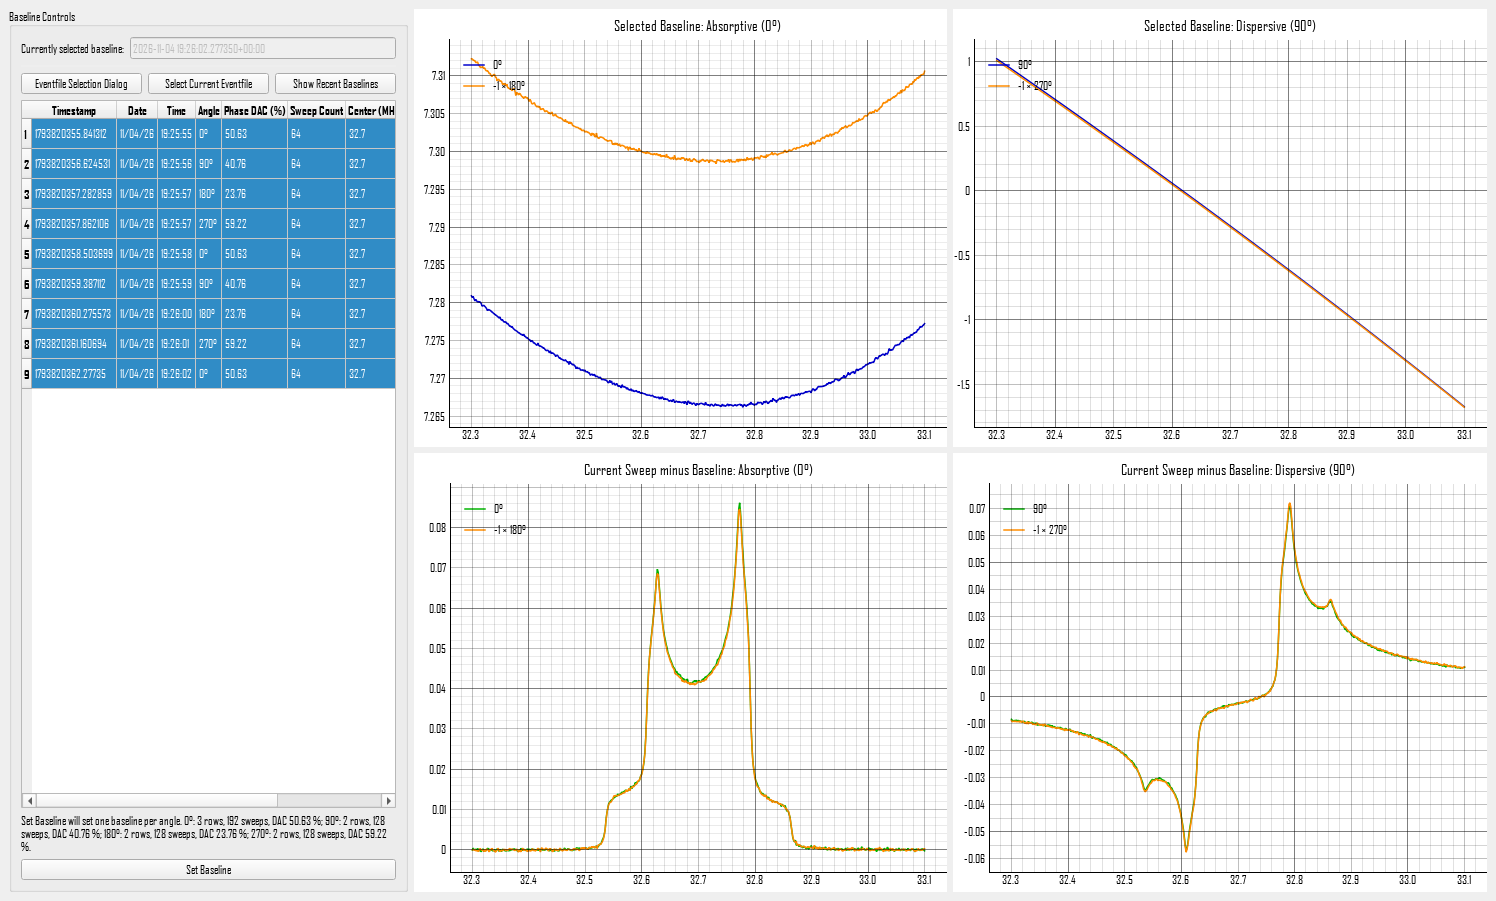
\includegraphics[width=\textwidth]{fig_baseline_tab.png}
\caption{The Baseline tab in the simulator, with a whole cycle4 baseline run (9 rows) selected and set, after the
line has come back on. The Angle and Phase DAC columns follow Time. Above \btn{Set Baseline}, the summary lists what
each angle gets. Right: the $2\times2$ grid, absorptive on the left and dispersive on the right; Selected Baseline on
top (orange: $-1\times180^\circ$ and $-1\times270^\circ$), Current Sweep minus Baseline below, where the opposite
settings overlay their partners.}
\label{fig:base}
\end{figure}

\subsection{Background subtraction for $90^\circ$ and $270^\circ$ records}
\label{sec:disp}
The Analysis tab's subtraction fits a polynomial to the wings and subtracts it. That suits the absorption,
which is small in the wings. The dispersion falls off only as $1/(f-f_L)$, so its tails reach the edges of the
window, and a wing fit takes part of them for background. In the 2026-10-27 hall data a cubic wing fit ate the
dispersion's tails, while a cubic fitted jointly with the Kramers--Kronig transform of the absorption, over the
whole sweep, left a dispersion that matched it to the noise.

PyNMR now does the second for every $90^\circ$ and $270^\circ$ record:
\begin{equation}
  y(f)=\sum_{j=0}^{3}c_j x^j + s\,\mathcal{H}[A](f),
\end{equation}
where $y$ is the baseline-subtracted sweep, $x$ the frequency scaled to $\pm1$ across the window, $A$ the
absorption of the latest $0^\circ$ record of the same run (averaged with $-1\times$ the $180^\circ$ record of the
same cycle in cycle4), $\mathcal H$ the Hilbert transform, and $s$ a free scale (the gain ratio and the sign of
$90^\circ$ go into it). Only the cubic is subtracted, so Fit Subtracted keeps the whole measured dispersion. The
fitted $s\,\mathcal H[A]$ is drawn dashed on the Fit Subtracted Imag plot as a check: with a good Imag tune the
two lie on top of each other, and $|s|$ is the gain ratio (about 1).
\begin{itemize}
\item $0^\circ$ and $180^\circ$ records keep the Analysis tab's subtraction.
\item The first dispersive record of a run, before any $0^\circ$ record, uses the wing fit;
  \code{quad\_sub\_method} records which was used.
\item The part of the dispersion due to absorption outside the window can't be predicted from inside it; it is
  smooth and goes into the cubic.
\item \code{dispersion: joint\_kk: False} in \code{quadrature.yaml} goes back to the wing fit for every angle.
\end{itemize}

\subsection{The plots}
\label{sec:plots}
While Quadrature is ticked, a $2\times3$ grid replaces the three plots under the Run tab (Fig.~\ref{fig:run}).
\begin{itemize}
\item The columns are the processing stages: Raw Signal, Baseline Subtracted, Fit Subtracted.
\item The top row is Real ($0^\circ$), the bottom row Imag ($90^\circ$).
\item In cycle4, $-1\times$ the $180^\circ$ record is drawn in orange over every $0^\circ$ plot, and
  $-1\times$ the $270^\circ$ record over every $90^\circ$ plot, so the opposite settings can be compared at a glance.
  On the Raw row they sit apart by twice the detector's DC offset; that gap \emph{is} the offset.
\item Baseline Subtracted shows the fitted background (yellow), with the points it was fitted to dashed red
  (\S\ref{sec:wings}).
\item Fit Subtracted: the solid purple line is the Analysis tab's result curve (JLab's; flat at zero for the
  default \emph{Integrate Full Range}, a fitted lineshape for the fitting methods). The dashed purple on Imag is the
  fitted KK curve (\S\ref{sec:disp}).
\item A raw curve follows its event live as the sweeps come in. Every other curve changes only when a record
  at its own angle finishes, so all of them can be watched as the line changes.
\item The big polarization number keeps showing the last Real record. The Signal Area box shows one line per
  angle, each from that angle's latest record, and changes only when a record at that angle finishes.
\end{itemize}
Unticking Quadrature shows JLab's three plots again.

\begin{figure}[ht]
\centering
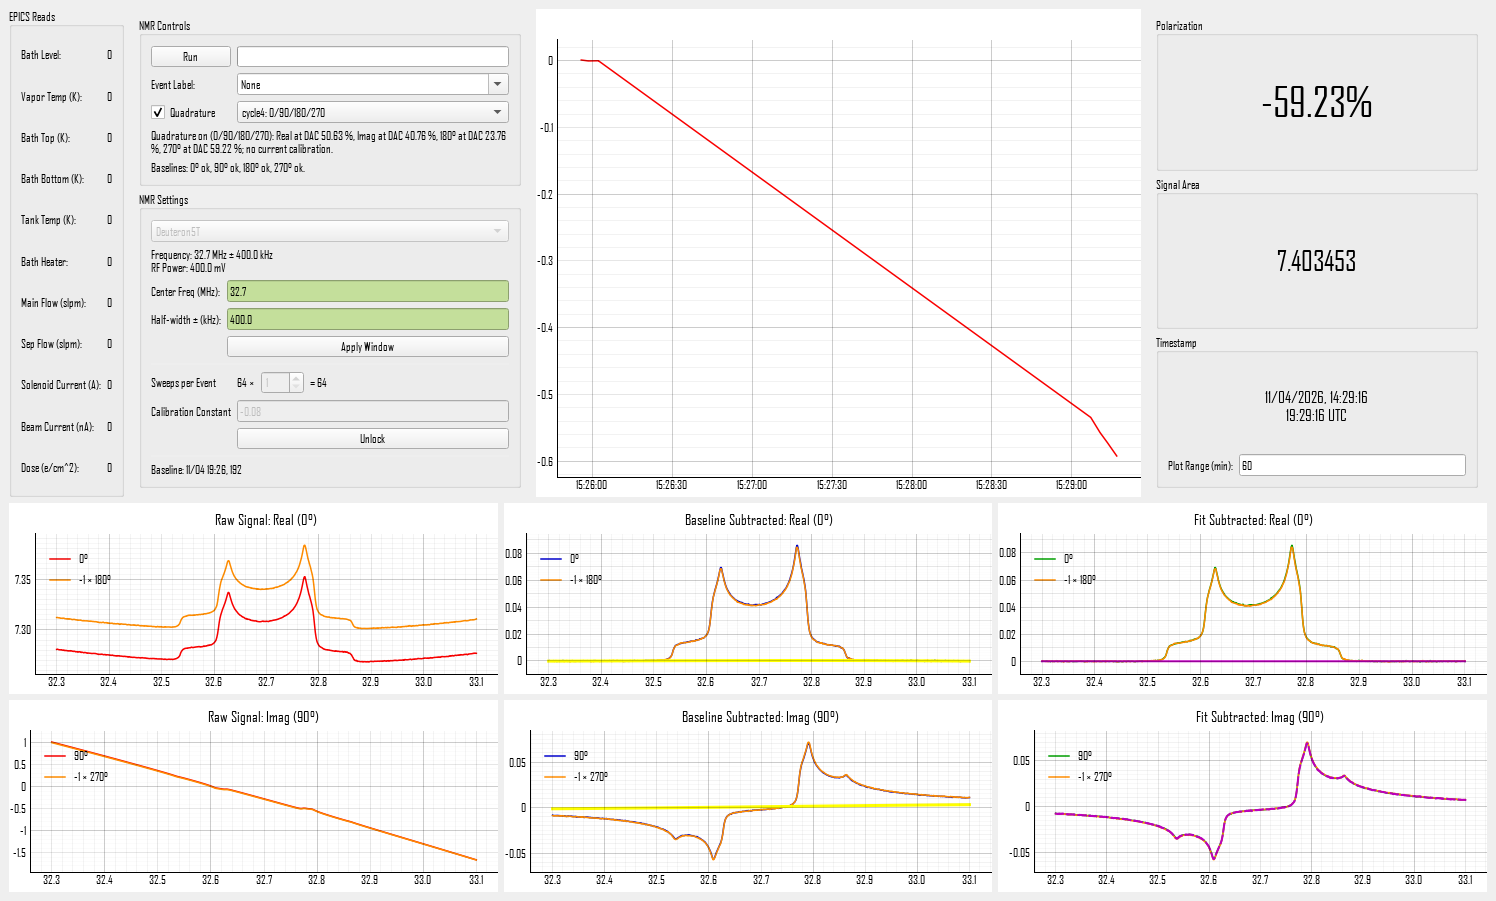
\includegraphics[width=\textwidth]{fig_run_tab_cycle4.png}
\caption{The Run tab during a cycle4 run in the simulator (Sweeps per Event $64\times1$), after a cycle4 baseline
set was selected in one go. Bottom: the $2\times3$ quadrature grid, with $-1\times180^\circ$ and $-1\times270^\circ$ in
orange. On the Raw row the gap between $0^\circ$ and $-1\times180^\circ$ is the simulated detector offset; each
angle's own baseline removes it. Fit Subtracted Imag shows the whole dispersion, tails included, with the fitted
KK curve dashed on top of it (here $s=1.01$).}
\label{fig:run}
\end{figure}

\subsection{Where the records go}
\begin{itemize}
\item \textbf{Event file:} every record, at every angle, with the \code{quad\_*} fields of Table~\ref{tab:fields}.
\item \textbf{EPICS and history (pol plot, TE tab):} $0^\circ$ records only. The area and polarization of
  $90^\circ$, $180^\circ$ and $270^\circ$ records are not polarizations.
\item \textbf{Online fitter:} $0^\circ$ records only.
\end{itemize}

\begin{table}[ht]
\centering\small
\begin{tabularx}{\textwidth}{@{}lX@{}}
\toprule
Field & Meaning \\
\midrule
\code{quad\_ref\_deg} & nominal angle: 0, 90, 180 or 270 \\
\code{quad\_vout} & phase DAC value for this record (equal to \code{phase\_vout}) \\
\code{quad\_tunes} & all tunes in use, e.g.\ \code{\{"0": 0.514, "90": 0.444, ...\}} \\
\code{quad\_mode}, \code{quad\_sequence} & \code{pair}/\code{abba}/\code{cycle4}/\code{custom}, and the list of angles \\
\code{quad\_group}, \code{quad\_index} & one pass through the sequence, and the position in it; pair records by group \\
\code{quad\_state} & \code{ok}, or \code{suspended} if the box refused a DAC write (the rest of the run is Real only) \\
\code{quad\_dac\_ok}, \code{quad\_dac\_set} & whether the box accepted the write, and which path set the tune \\
\code{quad\_settle\_ms} & wait after the DAC write \\
\code{quad\_cal\_id}, \code{quad\_cal\_valid} & calibration in force, and whether it covers these tunes \\
\code{quad\_cal\_angle\_deg}, \code{quad\_cal\_gain} & fitted angle and gain of this tune relative to Real \\
\code{quad\_base\_ref\_deg} & angle of the baseline subtracted (null for an untagged baseline) \\
\code{quad\_base\_vout}, \code{quad\_base\_match} & phase DAC the baseline was taken at, and whether it is this tune \\
\code{quad\_sub\_method} & $90^\circ$/$270^\circ$ records: \code{joint KK}, or the wing fit and why \\
\code{quad\_kk\_scale}, \code{quad\_kk\_curve} & fitted scale $s$ and $s\,\mathcal H[A]$ (dispersive records) \\
\bottomrule
\end{tabularx}
\caption{Quadrature fields on each event record.}
\label{tab:fields}
\end{table}

\paragraph{Offline.} With cycle4, Eq.~\eqref{eq:pairs} gives $I$ and $Q$ free of offsets. With a pair at a known
angle $\delta$ and gain ratio $g$ (from the calibration),
$I=P_0-o_0$ and $Q=\big[(P_\delta-o_\delta)/g-I\cos\delta\big]/\sin\delta$; the noise penalty is only
$1/\sin\delta$, so $\delta$ need not be exactly $90^\circ$. The first hall data (2026-10-27) showed the measured
dispersion matching the Kramers--Kronig transform of the absorption to about the noise, once the Q-curve
background was fitted jointly with it.

%=====================================================================================================
\section{Taking and using a TE}
\label{sec:te}
A thermal-equilibrium (TE) measurement calibrates the polarization: at a known temperature $T$ and field $B$ the
polarization is the Boltzmann value $P_\mathrm{TE}(B,T)$, so the calibration constant is
$\mathrm{CC}=\langle P_\mathrm{TE}/\mathrm{area}\rangle$, and every later event gets $P=\mathrm{area}\times\mathrm{CC}$.
The numbers below match the markers in Fig.~\ref{fig:te}.
\begin{enumerate}
\item \textbf{Take the TE data} (Run tab). Microwaves off, target at thermal equilibrium at a steady, known
  temperature; the EPICS temperature channel (\code{epics\_temp}, \code{TGT:PT12:Bath\_Top\_T} by default) must be live,
  because the TE uses its reading for each event. Use the same window, sweeps, baseline and Analysis-tab settings
  you will use for polarized data: the CC converts \emph{this} area to polarization. Set the Event Label to
  \textbf{TE} (the TE tab lists only events labelled TE or None) and run long enough to average the small signal.
  In quadrature only the $0^\circ$ records reach the history, so the TE uses Real records only.
\item \textbf{TE tab, Area vs.\ Time:} set \btn{History to Show (min)} to cover the TE, and drag the blue region over
  it. The line above reports an exponential fit (relaxation time and asymptote) to judge whether equilibrium was
  reached.
\item \textbf{Select for TE:} the lower plot shows the blue selection; drag the green region over the flat,
  equilibrium part. The fitted slope is shown above the table and should be consistent with zero.
\item \textbf{The points} appear in the table with their area and temperature. Double-click a row to drop an
  outlier. Points without a temperature reading are refused.
\item \textbf{Species and field:} choose \btn{Deuteron} (the box starts on Proton) and enter the field in T.
\item \btn{Calculate TE from Points}: TE Results shows the average TE polarization and CC, with spreads.
\item \btn{Save Results \& Use CC}: the report is written to \code{te\_dir} (default \code{te/}, created if needed) and the
  CC is put in use. The Run tab's Calibration Constant box shows it, and it is saved in the session.
\end{enumerate}

\begin{figure}[ht]
\centering
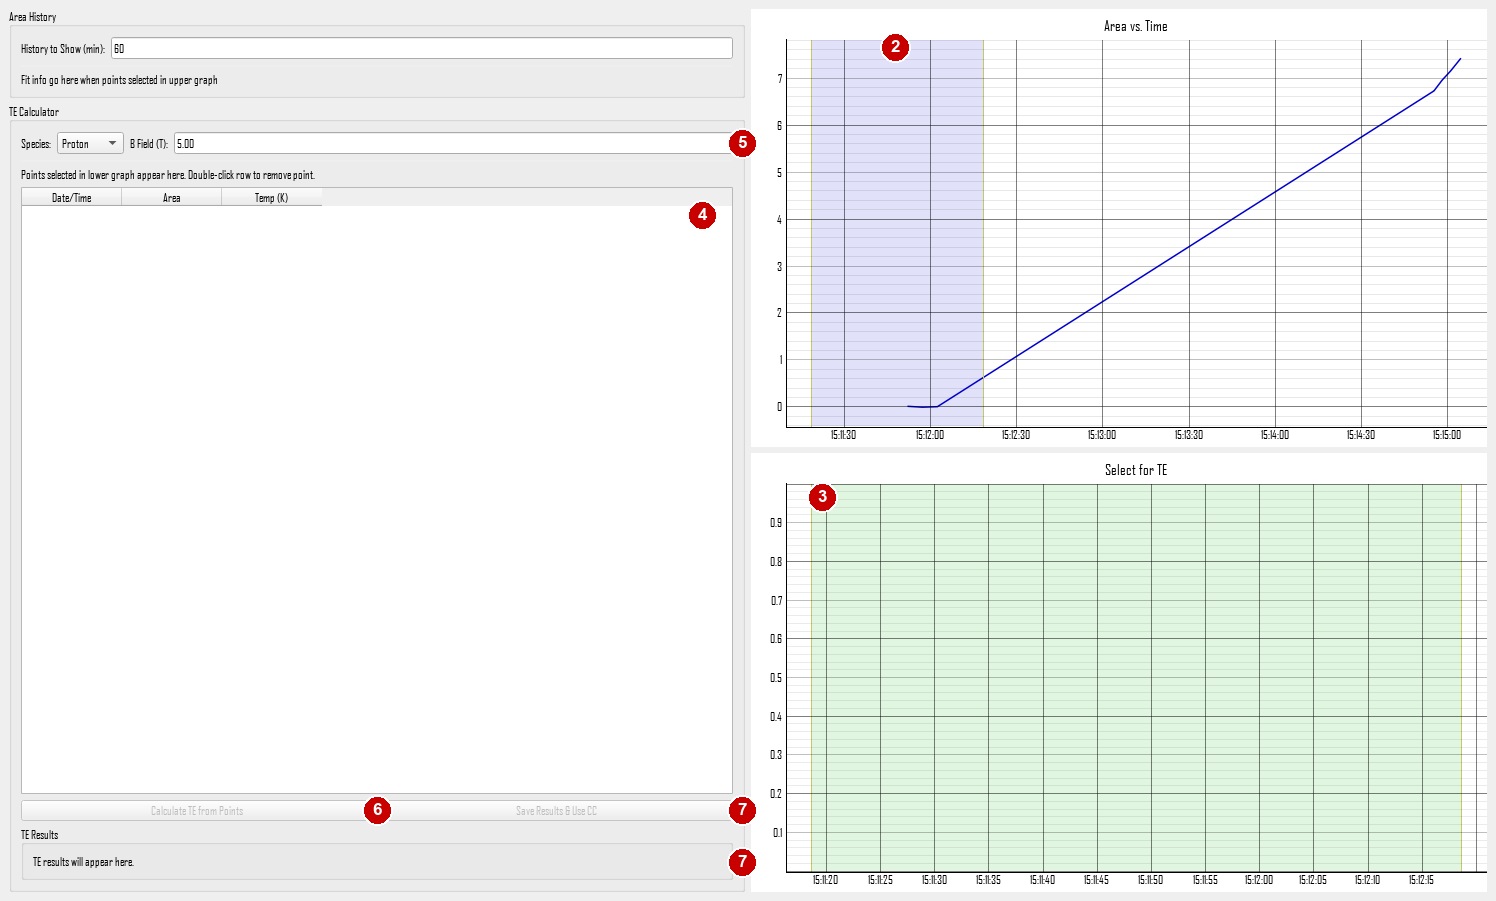
\includegraphics[width=\textwidth]{qs_te_marked.png}
\caption{The TE tab (simulator, so no temperatures and no points selected). \mk{2} Area vs.\ Time with the blue
selection. \mk{3} Select for TE with the green selection. \mk{4} the selected points. \mk{5} Species and B Field.
\mk{6} \btn{Calculate TE from Points}. \mk{7} \btn{Save Results \& Use CC} and the TE Results.}
\label{fig:te}
\end{figure}

%=====================================================================================================
\section{The Analysis tab}
\label{sec:analysis}
The Analysis tab sets how every event is analysed, in three stages: subtract a baseline, subtract a fitted
background, and turn what is left into a result (the area). Changing anything re-analyses the last event on this
tab at once, so the effect can be judged, and applies to every later event; records already written keep what
they had. Numbers match Fig.~\ref{fig:analysis}.
\begin{enumerate}
\item \textbf{Baseline Options:} \emph{Baseline Selected from Baseline Tab} (normal), \emph{Polynomial Fit to Wings}
  (fit the raw sweep's wings instead of using a baseline), or \emph{No Baseline Subtraction}.
\item \textbf{Subtraction Options:} \emph{Polynomial Fit to Wings} (normal) or \emph{No Fit Subtraction}.
\item \textbf{Polynomial order} (2nd to 8th; 3rd by default) and \textbf{Fit bounds (0 to 1)}: the two wing regions as
  fractions of the sweep. The Run tab's \btn{Wing bins} box sets these bounds (\S\ref{sec:wings}).
\item \textbf{Result Options:} \emph{Integrate Full Range} (default: the area is the sum of Fit Subtracted),
  \emph{Integrate within Range}, \emph{Peak Height}, \emph{Fit Gaussian and Integrate}, \emph{Fit 2 Gaussians and
  Integrate}, \emph{Deuteron Peak Fit} (JLab's lineshape fit; slower, up to about 25~s per event), or the two
  UNH options below.
\item[] \textbf{Optimized McClellan Fits (Equilibrium)} and \textbf{(ssRF)} run the online fitter's own fits
  (the \code{FitEngine} of LabView-NMR-Fitter, imported from the sibling folder) on each event, fed exactly as the
  data streamer feeds the fitter.
  \begin{itemize}
  \item \emph{Equilibrium} is the fast fit: r and the phase float, a cubic is profiled out, and every lineshape
    constant, \emph{including the amplitude scale}, is held fixed; $P=(r^2-1)/(r^2+r+1)$ (ratio method, no CC needed).
  \item \textbf{Press Update Constants} once about ten equilibrium lines are in, on a strong, steady line: it runs the
    full open fit on their average and refreshes all constants. Until then the status line is red and P is not
    trustworthy (in the simulator the preset amplitude was 1.6 times too small and P came out 1.7 times too high).
    Constants taken on weak lines (a few \%) are poor: re-run it once the signal is strong. The constants are saved
    in \code{<event\_dir>/mcclellan/} and reloaded at the next start for the same material.
  \item \emph{ssRF} is the fitter's hole-burnt fit against the Update-Constants reference; run Update Constants on the
    equilibrium line the manipulation starts from. Not yet tested inside PyNMR (the simulator burns no holes).
  \item Material: ND3, d-butanol or d-propanediol (\code{unh/mcclellan.yaml}). In quadrature only $0^\circ$ records are
    fitted. The fitter's fast fit misreads small \emph{negative} P (around $-5$ to $-15\,\%$) as positive; this is a
    property of the fitter, reported to its maintainers.
  \end{itemize}
\item \textbf{Plots:} Baseline Subtraction (raw, baseline, difference); Fit Subtraction, with the wing regions shaded;
  Results, with the result curve (the purple line on the Run tab).
\end{enumerate}
\begin{itemize}
\item The CC from a TE is valid only for the analysis settings used during that TE. Change them and take a new TE.
\item In quadrature, $90^\circ$ and $270^\circ$ records use the joint KK subtraction (\S\ref{sec:disp}) instead of
  step~2's choice. Re-analysis on this tab uses the tab's own choice for every record, for display.
\end{itemize}

\begin{figure}[ht]
\centering
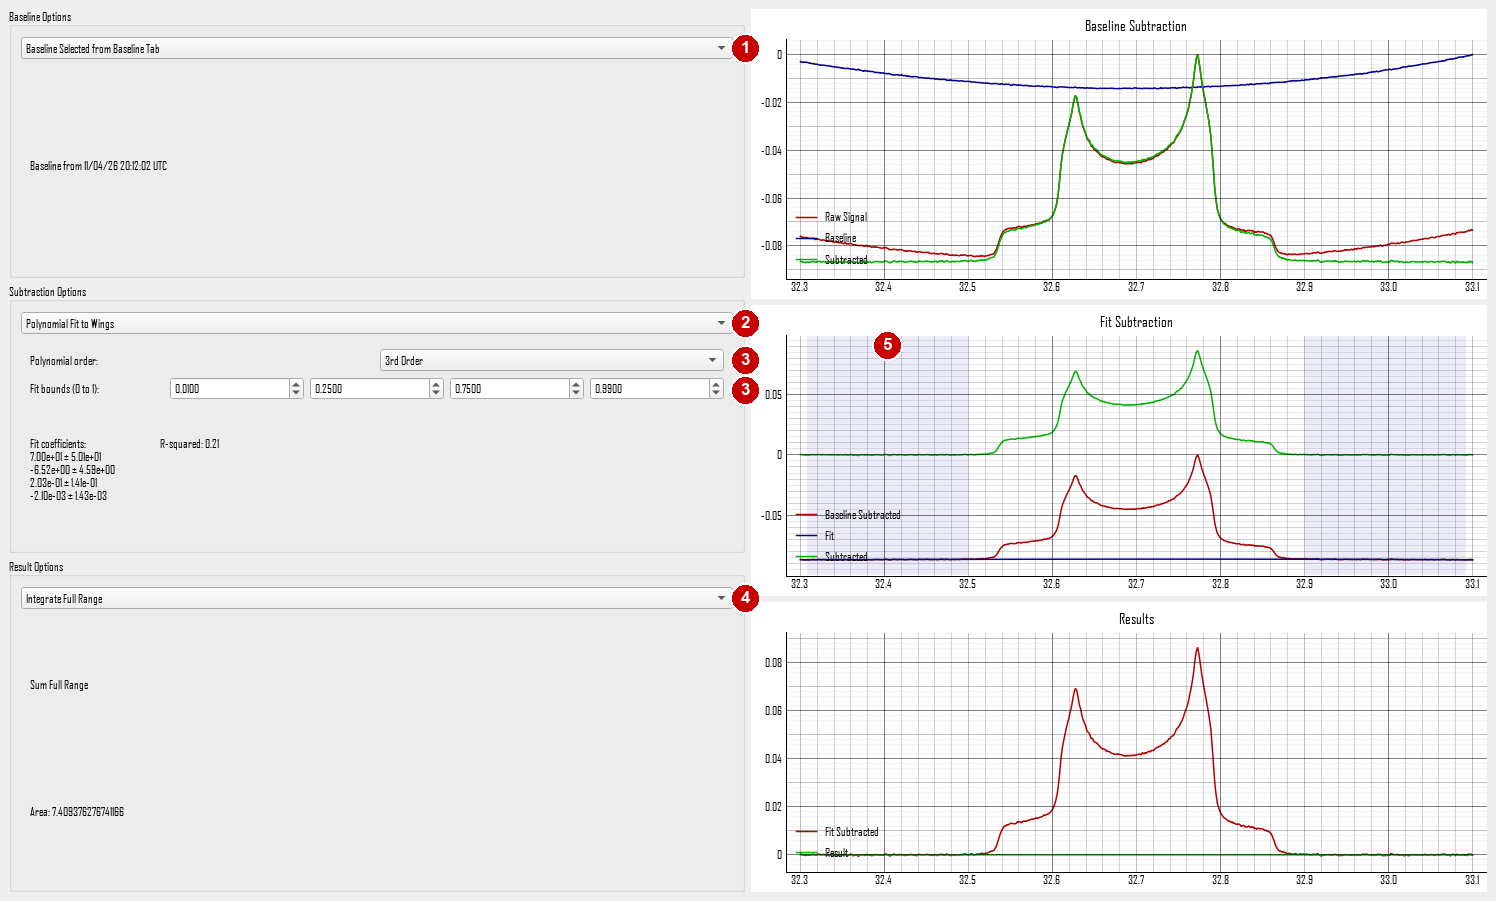
\includegraphics[width=\textwidth]{qs_analysis_marked.png}
\caption{The Analysis tab. \mk{1} baseline method. \mk{2} subtraction method. \mk{3} polynomial order and fit bounds.
\mk{4} result method. \mk{5} the shaded wing regions on the Fit Subtraction plot.}
\label{fig:analysis}
\end{figure}

%=====================================================================================================
\section{Troubleshooting}
\label{sec:trouble}

\begin{table}[ht]
\centering\small
\begin{tabularx}{\textwidth}{@{}>{\raggedright\arraybackslash}p{0.33\textwidth}X@{}}
\toprule
Symptom & What to do \\
\midrule
Quadrature box won't tick & Read the red line beside it: set the named tune on the Tune tab, or move it off the Real tune's DAC value. \\
Box stops answering (``Exception starting DAQ connection: timed out'') & Power cycle the box, then restart PyNMR. It happens when PyNMR dies mid-sweep; check you're on \code{pynmr312}. \\
Quadrature suspended mid-run & The box refused a DAC write; the rest of the run is Real only. Check the log, restart the run. \\
``no current calibration'' & The tunes, channel or window changed since the last calibration. The data are fine; run \btn{Auto Calibrate Phase} if you need recorded angles. \\
\btn{Auto Tune} not converged & Set the tunes closer by hand (within about $30^\circ$) and try again. \\
\btn{Auto Tune} result looks wrong & \btn{Undo Auto Tune}. Check the trace plot: a messy trace, or a strong deuteron line, can bias it; try \code{mask\_khz}. \\
Event of 640 sweeps times out with Quadrature on & Should no longer happen (DAC now written between events); report it with the log. \\
Baselines line in red & ``none'': select a baseline set that includes that angle. ``taken at another tune'': the
tune moved (Auto Tune); take a new baseline set. \\
Imag Fit Subtracted has odd wings & Check \code{quad\_sub\_method} is \code{joint KK} and the dashed KK curve follows the
data; a baseline from another tune or a poor $0^\circ$ record shows up here. \\
Fitter not updating & Is it running? PyNMR logs one warning per outage and keeps going. Only $0^\circ$ records are sent. \\
\bottomrule
\end{tabularx}
\caption{Common problems.}
\end{table}

%=====================================================================================================
\section{Status and limits}
\begin{itemize}
\item \textbf{Tested on the box (2026-10-27):} quadrature alternation, cycle4, the calibration, the per-angle
  records. 16 complete cycle4 groups were taken on the deuteron line.
\item \textbf{Simulator only so far:} \btn{Auto Tune}, the $2\times3$ plots, per-angle baseline selection, the joint-KK
  background for dispersive records, the $64\times N$ sweep controls, 64-sweep tune chunks, the default tunes, and
  the fix for 640-sweep timeouts.
\item The $90^\circ$ angle rests on the smooth-gain assumption; $0^\circ$ and $180^\circ$ don't.
\item The absorptive phase turns across the window by the Q-curve's arc. \btn{Auto Tune} makes the reference
  absorptive at the centre frequency; the offline complex fit handles the rest.
\end{itemize}

%=====================================================================================================
\appendix
\section{Why the Q-curve fixes the absorptive phase}
\label{app:normal}

For the constant-current (Liverpool) Q-meter, the detected voltage is a fixed function of the tank impedance,
$V=F(Z)$ with $F(Z)=U Z/(R_{cc}+Z)$, and $Z=R+iX(f)$. Sweeping the frequency changes the reactance $X$;
absorption by the sample adds to the coil's resistance $R$ (in proportion to $\chi''$). So
\begin{equation}
  \frac{dV}{df}=F'(Z)\; i\,X'(f), \qquad \frac{dV}{d\chi''}\;\propto\;F'(Z)\;\frac{dR}{d\chi''}.
\end{equation}
Both share the factor $F'(Z)$; one is multiplied by an imaginary number and the other by a real one. The NMR
absorption at frequency $f$ therefore points along the \emph{normal} to the Q-curve's trace at $f$, and the
dispersion along the trace itself. The same holds with the $\lambda/2$ cable between tank and coil, to the
extent that the cable's own frequency dependence is small over the window.

Because $F$ is a M\"obius map and $X$ is close to linear in $f$, the trace is a circle (or, for large $R_{cc}$, a
nearly straight line), and the angle about its centre runs as
\begin{equation}
  \theta(f)=\theta_0+2\arctan\!\left(\frac{f-f_0}{\gamma}\right),
\end{equation}
with $f_0$ the resonance ($X=0$) and $\gamma=(R_{cc}+R)/X'$ the width of the trace's parametrization, which
is wider than the tank's own half-width $R/X'$. The normal turns with it, so this is also the absorptive
phase at each frequency: the form found experimentally by E.~Long years ago.
Figure~\ref{fig:normal} checks this in the simulator's Q-meter with a Q~$\approx26$ tank like the Hall~B one:
the normal and the true absorption direction agree to better than $10^{-6}$ degrees at every frequency, and
both turn by about $19^\circ$ across a $\pm200$~kHz window.

\begin{figure}[ht]
\centering
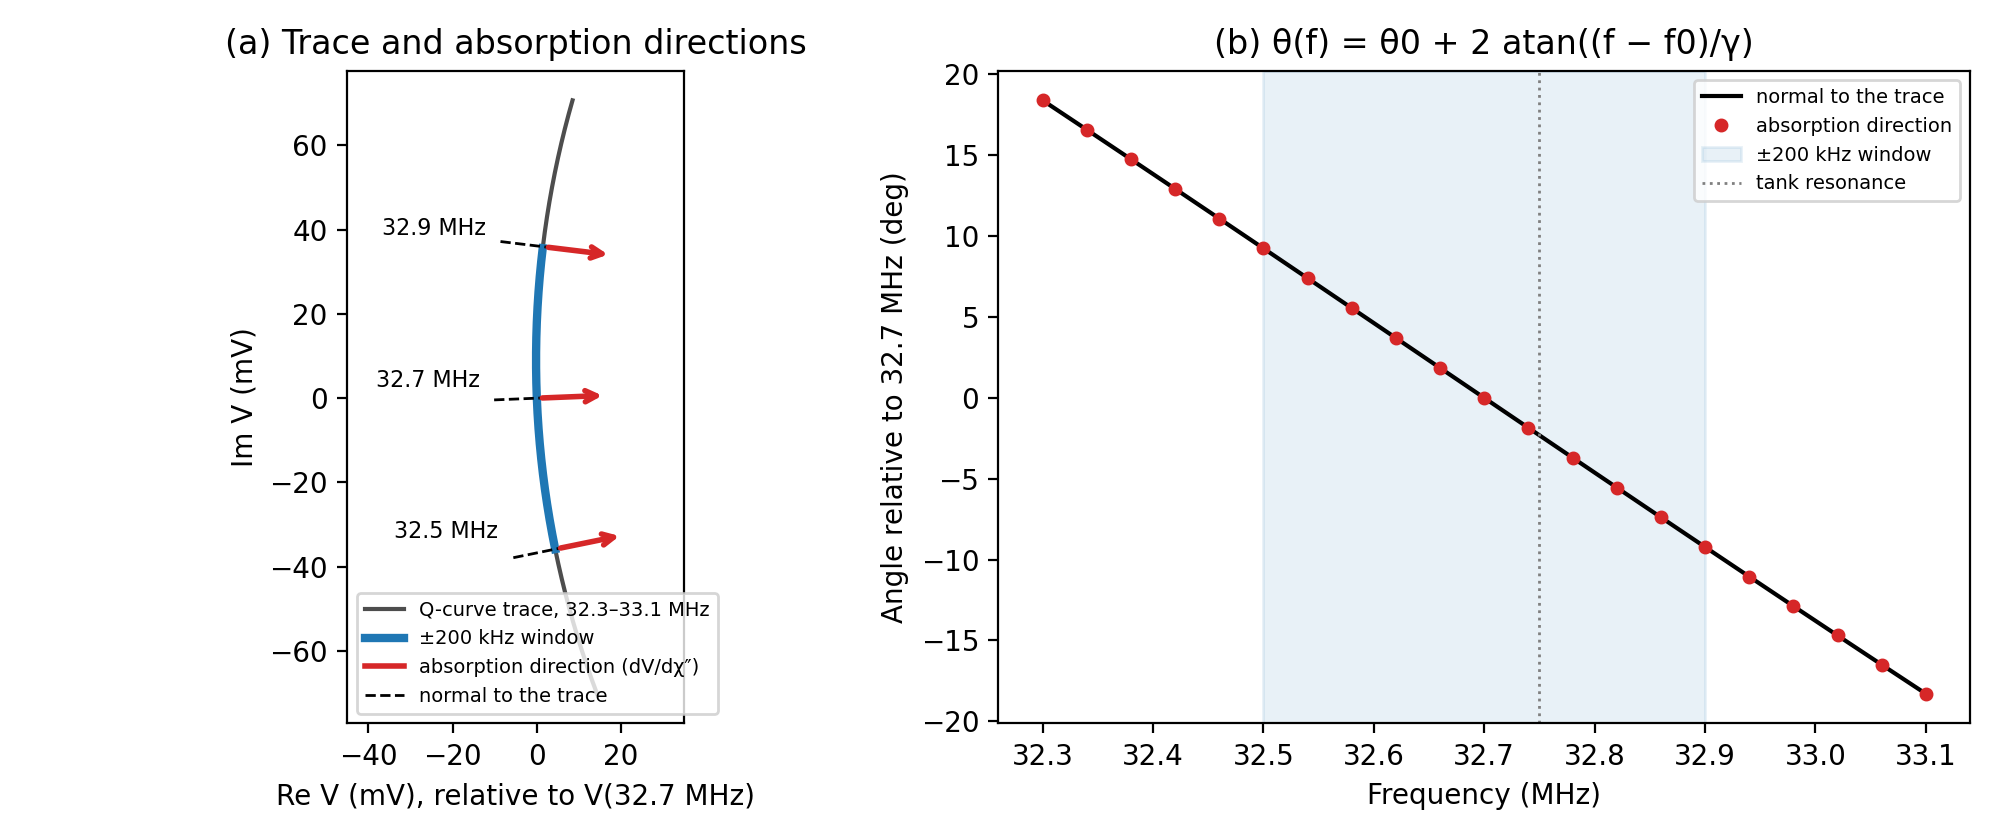
\includegraphics[width=\textwidth]{fig_trace_normal.png}
\caption{Simulated Q~$\approx26$ tank ($R_{cc}=50~\Omega$, tank resonance 50~kHz above the window centre).
(a)~The Q-curve trace with the true absorption direction $dV/d\chi''$ (red arrows) and the normal to the trace
(dashes) at three frequencies. (b)~Both angles across the sweep, relative to 32.7~MHz.}
\label{fig:normal}
\end{figure}

\paragraph{Why the centre frequency and not the resonance.} A $\pm200$~kHz window covers a small part of the
trace (about $\pm0.08\,\gamma$ for the Q~$\approx26$ circuit, where $\gamma\approx2.5$~MHz), so $f_0$ is poorly determined: in a Q~$\approx26$ test, the
normal taken at the fitted $f_0$ was $4^\circ$ off. The normal at the centre frequency needs no $f_0$ and is
where the line sits. Across three test circuits (a straight trace, the Q~$\approx26$ circle, and a circle with a
$\lambda/2$ cable) and tank detunings up to 200~kHz, it matched the true absorption direction within $0.5^\circ$.

\section{The Auto Tune algorithm}
\label{app:algo}
Code: \code{unh/quadrature/autotune.py} (fits) and \code{AutoTuneThread} in \code{unh/quadrature/calibration.py}.
\begin{enumerate}
\item \textbf{Local calibration.} The steps around the tunes are fitted with the calibration model
  \[
  y_{kj}=g(v_k)\,(1+d\,\tau_k)\big[\mathrm{Re}\,W_j\cos\phi_k+\mathrm{Im}\,W_j\sin\phi_k\big]+o(v_k),
  \]
  with the phase $\phi$ free at every DAC value ($\phi=0$ at the Real tune), $g$ and $o$ low-order polynomials in
  $v$, a linear drift $d$, and $W_j$ the complex response in 32 frequency bins.
\item \textbf{Trace fit.} The points $W_j=x_j+iy_j$ are fitted geometrically with a circle written as a conic,
  \[
  A\,(x^2+y^2)+B\,x+C\,y+D=0,\qquad B^2+C^2-4AD=1\ \text{(Pratt)},
  \]
  which stays finite as the circle straightens into a line ($A\to0$). The normal at the point for the centre
  frequency is the gradient, $\theta_\mathrm{ref}=\operatorname{atan2}(2Ay+C,\;2Ax+B)$; its error comes from a
  jackknife over the bins, folded mod $180^\circ$. In the simulator it is within $0.45^\circ$ of the truth, and
  the points scatter off the curve by about the noise. (An earlier fit of the circle's parametrization in $f$
  followed the trace poorly.)
\item \textbf{Targets.} $0^\circ$ is whichever of $\theta_\mathrm{ref}$ and $\theta_\mathrm{ref}+180^\circ$ is nearer the
  hand Real tune; $90^\circ$ is whichever of $\theta_\mathrm{ref}\pm90^\circ$ is nearer the hand Imag tune;
  $180^\circ$ and $270^\circ$ are opposite those.
\item \textbf{DAC values.} Around each tune, a quadratic $\phi(v)$ through the five settings is solved for the
  target. If the answer lies outside them, another pass is centred on it (at most \code{max\_passes}, 3).
\item \textbf{Polish.} Once every target lies inside its settings, one more pass with \code{polish\_offsets}
  ($\pm0.5$ and $\pm1$\,\%) is centred on the new tunes, and its answer is final. The spacing of the settings
  doesn't set the precision (the fit through them does); the polish measures the final tunes directly and
  shrinks any error from the shape assumed for $\phi(v)$.
\end{enumerate}
Settings are under \code{autotune:} in \code{quadrature.yaml}: \code{offsets}, \code{sweeps\_per\_step} (64),
\code{max\_passes}, \code{polish}, \code{polish\_offsets}, \code{bins}, \code{gain\_order}, \code{offset\_order}, \code{fit\_drift} and \code{mask\_khz}.

\end{document}
